\label{section:2d_hillslope_example}
This example \footnote{See verification example   \texttt{MUT\_Examples$\backslash$2\_VSF\_Hillslope}} simulates variably-saturated flow in a 2D hillslope of homogeneous material which receives a uniform recharge rate of 1.27 x 10$^{-8}$ m/s was applied directly to the \gwf\ domain at the ground surface. .

These are the properties we used:

\begin{tabular} {ccc} \hline
    Variable name           &    Value        & Units \\ \hline
	Kh\_Kx:             &     1.0E-06 & m/s \\
	Kv\_Kz:             &    1.0E-06   & m/s \\
	Specific Storage:  &    1.0E-05   & 1/m \\
	Specific Yield:    &    0.1       & - \\
	Alpha:             &    3.34E-02   & 1/m \\
	Beta:              &     1.982       & 1/m \\
	Sr:                &    0.2771       & - \\ \hline
\end{tabular}

The Van Genuchten unsaturated function type was used.

 

A drain boundary condition was with a drain conductance of 1000 m/s was applied to the \gwf\ domain at the ground surface.


Here is the hydraulic head distribution at 242 years (equilibrium):
    \vspace{.2in} \\
    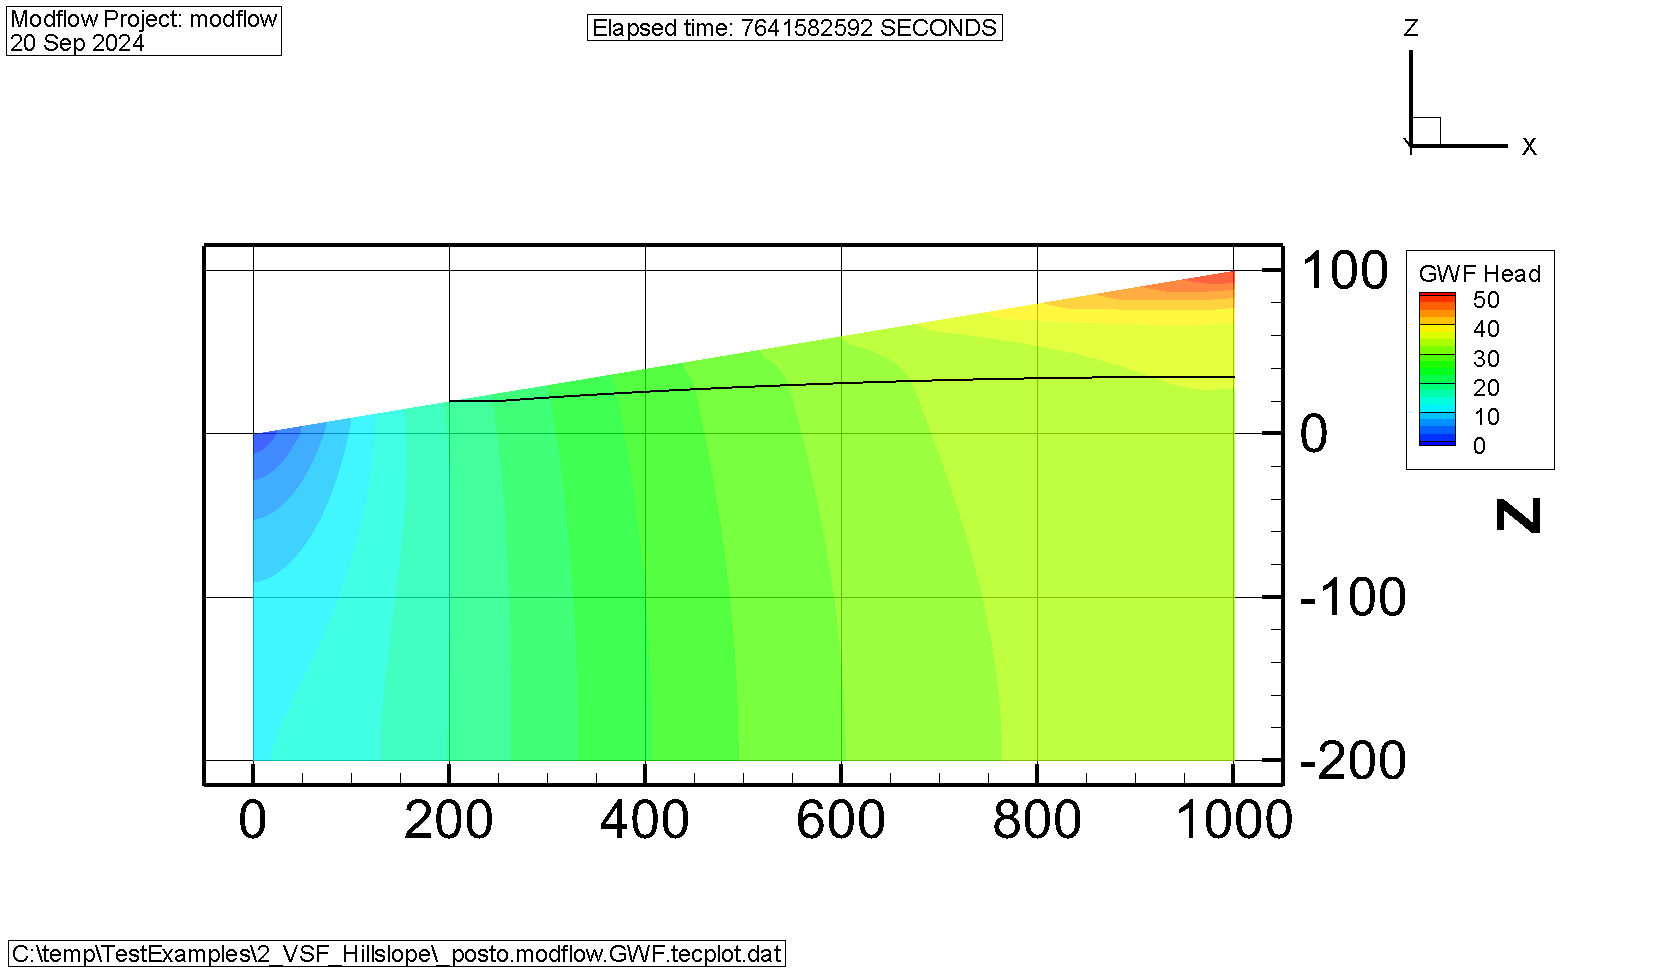
\includegraphics[width=0.97\textwidth]{2D_Hillslope_GWF_Head_and_water_table}
    \vspace{.2in} \\

Some key features of this example are:
\begin{itemize}
    \item The hill slopes from an elevation of 0 m at $x=0$ to 1000 m at $x=1000$.
    \item The base is flat at an elevation of -200 m.
  \item The water table is shown as heavy black line. 
\end{itemize}
